\pagebreak
\section{Edge Connectivity}
In this problem you will write a code that identifies loops of connected points given a scrambled list of edges. The assignment came with two files: {\tt{V.txt}}, which contains the $(x, y)$ coordinates of the points(nodes); and {\tt{E.txt}} which contains the list of edges.  Each line in {\tt{E.txt}} corresponds to one edge. It contains two integers, which are the node numbers (numbering starts at 1) of the two endpoints of that edge. The coordinates of node $n$ are given on line $n$ of {\tt{V.txt}}. A \textit{loop} is an ordered sequence of nodes in which the first and last nodes are the same, and each pair of consecutive nodes is connected by an edge. For a given loop, all of the provided edges have the node pairs numbered consistently(either clockwise or counterclockwise).

Write a code that reads in the two files and performs the following:
\begin{itemize}
    \item Prints out the number of loops
    \item Starting from the shortest loop and progressing to the longest, prints out the number of unique nodes and the list of nodes in each loop.  Start the list of nodes with the smallest-index node number.  Format the printing to show 10 numbers per line, with the numbers right-justified in aligned columns.
    \item Makes a plot of the loops by connecting the ordered nodes in each loop.  Use a different color and symbol for each loop.  You will find that one of the loops is much further away from the others, so make two plots, one with all of the loops, and one zoomed in to show all but the faraway loop.
\end{itemize}

In your writeup, explain your approach and algorithm, and include all of the requested output and plots.  The documented code should go in the {\tt.zip} file, but we should not have to run it to see the results.


\begin{adjustwidth}{2.5em}{0pt}

    \subsection*{Edge Connectivity Algorithm}
    \begin{enumerate}
        \item My algorithm in an overview has two nested while loops with {\tt{if}} conditional statements to determine the edge connectivity within the loops.
        \begin{itemize}
            \item First {\tt while} loop is used to loop through all the loops until the algorithm determines that it has found all the interior loops
            \item The seconds {\tt while} loop will loop through {\tt E.txt} to find which nodes belongs to the loop in question
        \end{itemize}
        \item Then while in these {\tt while} loops, inside I have two {\tt if} statements
        \begin{itemize}
            \item One {\tt if} statement is used to determine the next node that is connected within the interior loop
            \item The other {\tt if} statement is used to determine if it has looped through all the interior nodes and has reached back around to the beginning of the interior loop
        \end{itemize}
        \item Outside of the inner {\tt while} loop is another if statement that determines if there are values that still need to be looped over and if so it will pre-allocate values for when it loops through the next interior loop
        \item Then once finished with these loops printing the values is done through {\tt unique} and {\tt sort} and remove all 0 entries to remove the possibility of concatenation errors
    \end{enumerate}

    \begin{fminipage}{0.8\linewidth}
        \textbf{Implementing my above method, being more involved and extra variables, I was able to {\tt fprintf} to Matlab in the right-justified format with 10 numbers per line. However, the next page I output the values to Table \ref{tab:loop_results} as well. Code will be attached at the end of my assignment.}
    \end{fminipage}
\end{adjustwidth}


\begin{table}[h!]
    \centering
    \caption{Edge connectivity unique nodes per loop in ascending order.}
    \label{tab:loop_results}
    \begin{tabular}{ r | r | r | r | r | r | r | r | r | r }
        \input{q4/loop_results}
    \end{tabular}
\end{table}

\begin{fminipage}{0.8\linewidth}
    \textbf{Above in Table \ref{tab:loop_results} are the nodal values to the edge values for each given loop. Attached to the end is the tabulated output from Matlab Command Window.}
\end{fminipage}

\pagebreak
\begin{figure}[h]
    \centering
    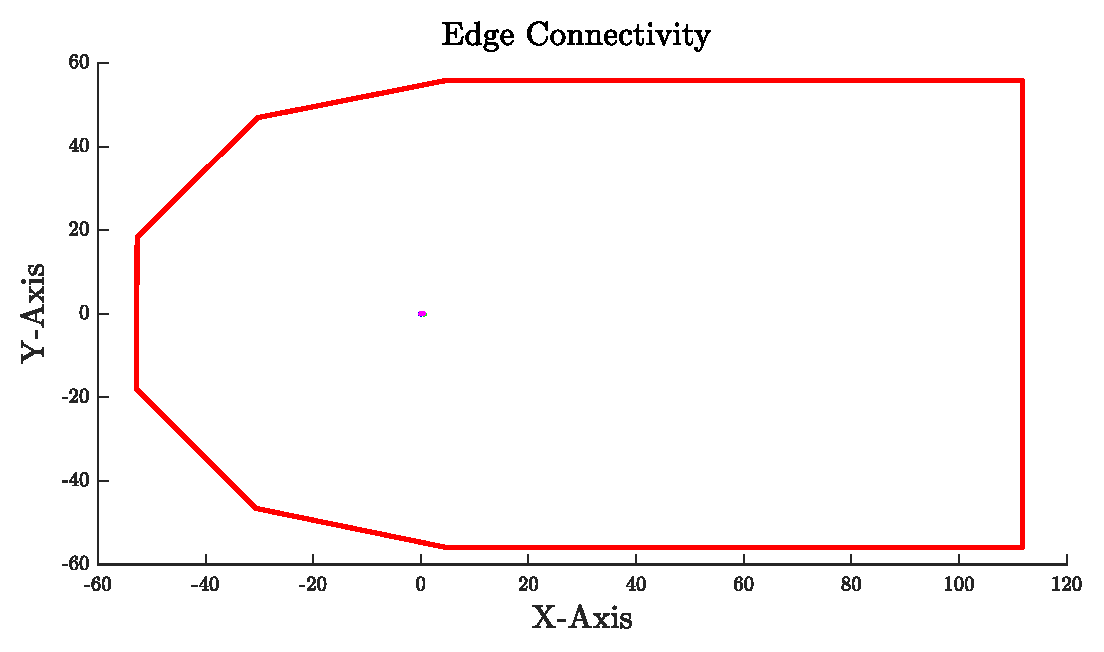
\includegraphics[width = 0.8\linewidth]{q4/big_loops.eps}
    \caption{Full view of all loops.}
    \label{fig:big_loops}
\end{figure}


\begin{figure}[h!]
    \centering
    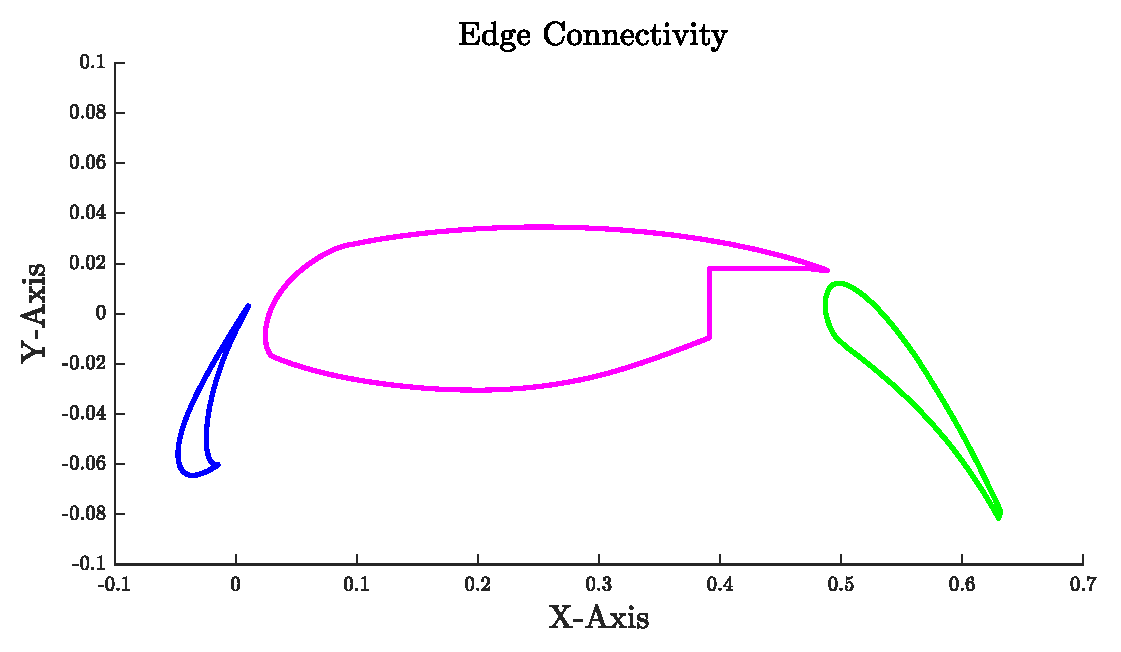
\includegraphics[width = 0.8\linewidth]{q4/small_loops.eps}
    \caption{Zoomed in view of all loops.}
    \label{fig:small_loops}
\end{figure}


\begin{fminipage}{0.8\linewidth}
    \textbf{Looking above to Figures \ref{fig:big_loops},\ref{fig:small_loops} I can see that my Matlab code correctly implemented the iterations to determine the correct loops and then succesfully tabulated them to the loops.}
\end{fminipage}